\title{Dokumentacja projektu}
\author{
	Krzysztof Mizgała 262839
	\and 
	Maciej Kosierb 262239
	\and
	Wiktoria Kudła 262254
	\and
	Wiktoria Gałdusińska 262209
}
\date{\today}

\documentclass[12pt]{article}
\usepackage[hidelinks]{hyperref}
\usepackage{polski}
\usepackage[utf8]{inputenc}
\usepackage{pgf-umlcd}
\usepackage{listings}
\usepackage{graphicx}
\usepackage{float}
\usepackage{xcolor}
\usepackage{xparse}

\NewDocumentCommand{\codeword}{v}{
	\texttt{\textcolor{blue}{#1}}
}

\begin{document}
	\maketitle
	\tableofcontents
	\newpage
	
	\section{Opis projektu}\label{sec:opis-projektu}
	Nasza aplikacja służy do analizy danych finansowych.
	Korzysta z danych z \underline{\href{https://site.financialmodelingprep.com/developer/docs/}{Financial Modeling Prep API}}.
	Klucz API jest wymagany do uruchomienia aplikacji.
	Można go pobrać \underline{\href{https://site.financialmodelingprep.com/login}{tutaj}} a następnie
	trzeba ustawić zmienną środowiskową API\_KEY do klucza.
	Można także korzystać z własnego klucza API tworząc plik .env w katalogu głównym projektu i
	dodając zmienną API\_KEY z kluczem jako wartość.

	Aplikacja pozwala na odczyt danych finansowych danej firmy.
	Używając różnych metod do zanalizowania, pokazuje wyniki i przewiduje ceny rynkowe.

	\section{Użyte technologie}\label{sec:uzyte-echnologie}

	 Wykorzystane biblioteki Pythona:
	\begin{itemize}
		\item pandas
		\item requests
		\item dotenv
		\item PyQt5
	\end{itemize}

	Lista plików:
	\begin{itemize}
		\item analysis.py
		\item api.py
		\item docs.tex
		\item README.md
		\item requirements.txt
		\item ui.py
	\end{itemize}

	\section{Opis metod}\label{sec:uzyte-metody}
	\subsection{ui.py}
		\begin{itemize}
			\item \codeword{_get_symbols} - pobiera symbole i nazwy analizowanych obiektów z pliku CSV.
			\item \codeword{_init_it} - tworzy graficzny interfejs użytkownika.
			\item \codeword{_update_symbols} - aktualizuje listę nazw instrumentów finansowych przy zmianie kategorii.
			\item \codeword{update_signal} - aktualizuje etykietę sygnału i kolor pudełka przy zmianie sygnału.
			\item \codeword{update_indicators} - aktualizuje listę wskaźników przy zaznaczaniu pól wyboru wskaźników.
			\item \codeword{update_bins} - aktualizuje liczbę słupków histogramu.
			\item \codeword{analyze} - analizuje dane dla wybranego obiektu.
			Pokazuje wyniki w postaci tabeli i wykresu świecowego.
			\item \codeword{_analyze} - zaczyna analizę w osobnym wątku po to, by zapobiec zacinaniu się interfejsowi.
			\item \codeword{draw_plot} - tworzy wykres świecowy.
			\item \codeword{plot_candles} - tworzy świece wykresu na osiach na podstawie dostarczonych danych.
			\item \codeword{plot_indicators} - tworzy wykres wskaźników, które zostały wybrane przez użytkownika, na wykresie
			świecowym.
			\item \codeword{plot_sma} - tworzy wykres wskaźników SMA na wykresie świecowym.
			\item \codeword{plot_ema} - tworzy wykres wskaźników EMA na wykresie świecowym.
			\item \codeword{plot_bollinger} - tworzy wykres wstęg Bollingera na wykresie świecowym.
			\item \codeword{plot_rsi} - tworzy wykres wskaźników RSI na wykresie świecowym.
			\item \codeword{plot_macd} - tworzy wykres wskaźników na wykresie świecowym.
			\item \codeword{plot_stochastic} - tworzy wykres oscylatora stochastycznego na wykresie świecowym.
			\item \codeword{plot_williams} - tworzy wykres \%R Williamsa.
		\end{itemize}
		\subsection{analysis.py}\label{wskazniki}
		\begin{itemize}
			\item \codeword{get_signal} - otrzymuje sygnał na opierający się na wskaźnikach analizy techniczej.
			Bazuje na następujących zasadach:
			\begin{itemize}
				\item Kupno, gdy MACD przekracza linię sygnału z góry.
				\item Sprzedaż, gdy MACD przekracza linię sygnału z dołu.
				\item Kupno, gdy RSI jest mniejszy niż 30.
				\item Sprzedaż, gdy RSI jest większy niż 70.
				\item Kupno, gdy \%K (oscylator wolny) przekroczy \%D (oscylator szybki).
				\item Sprzedaż, gdy \%D przekroczy \%K.
				\item Kupno, gdy SMA jest większe od EMA.
				\item Sprzedaż, gdy SMA jest mniejsze od EMA.
				\item Kupno, gdy SMA jest większe od ceny instrumentu.
				\item Sprzedaż, gdy SMA jest mniejsze od ceny instrumentu.
				\item Kupno, gdy EMA jest większe od ceny od ceny instrumentu.
				\item Sprzedaż, gdy EMA jest mniejsze od ceny instrumentu.
			\end{itemize}
			\item \codeword{sma} - Prosta Średnia Krocząca (ang. SMA - Simple Moving Average), jest
			najbardziej podstawową średnią kroczącą.
			Oblicza się ją sumując ceny zamykające z ostatnich\textit{n} dni i dzieląc tę sumę przez \textit{n}.
			\item \codeword{ema} - Wykładnicza Średnia Krocząca (ang. EMA - Exponential Moving Average) jest rodzajem
			średniej kroczącej, która kładzie większy nacisk na nowszych danych.
			EMA jest bardziej wrażliwy na ostatnie zmiany w cenie.
			\item \codeword{bollinger} - Wstęgi Bollingera to wstęgi zmienności między średnią krocząca.
			Zmienność jest liczona za pomocą odchylenia standardowego, które zmienia się, kiedy
			zmiennośc rośnie lub maleje.
			Wstęgi automatycznie poszerzają się, kiedy zmienność rośnie i zwężają, gdy maleje.
			\item \codeword{rsi} - Wskaźnik Siły Względnej (ang. RSI - Relative Strength Index) jest wskaźnikiem
			dynamiki, który mierzy znaczenie ostatnich zmian cen, aby ocenić warunki wykupienia lub wyprzedania
			akcji lub innego kapitału.
			\item \codeword{macd} - Konwergencja/Dywergencja Średnich Kroczących (ang. Moving Average Convergence Divergence)
			to wskaźnik dynamiki trendów pokazujący zaleźność pomiędzy dwiema średnimi kroczącymi cen.
			\item \codeword{stochastic} - Oscylator Stochastyczny (ang. Stochastic Oscillator) jest wskaźnikiem dynamiki,
			który porównuje konkretną cenę zamykającą do zakresu jej cen na przestrzeni czasu.
			\item \codeword{williams} - \%R Williamsa to wskaźnik dynamiki. Jest oscylatorem, który pokazuje zależność obecnej
			ceny zamknięcia w relacji do maksymalnej i minimalnej ceny z poprzednich dni.
		\end{itemize}
		\subsection{api.py}
			\begin{itemize}
				\item \codeword{_get_data} - tworzy ramkę danych lub plik JSON z danych z API dla danego adresu URL.
				\item \codeword{list_category} - tworzy listę symboli danej kategorii.
				\item \codeword{get_historical} - pobiera ceny historyczne oraz wolumen dla danej akcji, kryptowaluty, forexa lub zasobu.
				\item \codeword{get_historical_capitalization} - pobiera kapitalizację historyczną dla konkretnego symbolu.
				akcji.
			\end{itemize}

\newpage
	\section{Diagram UML}\label{sec: diagram}
	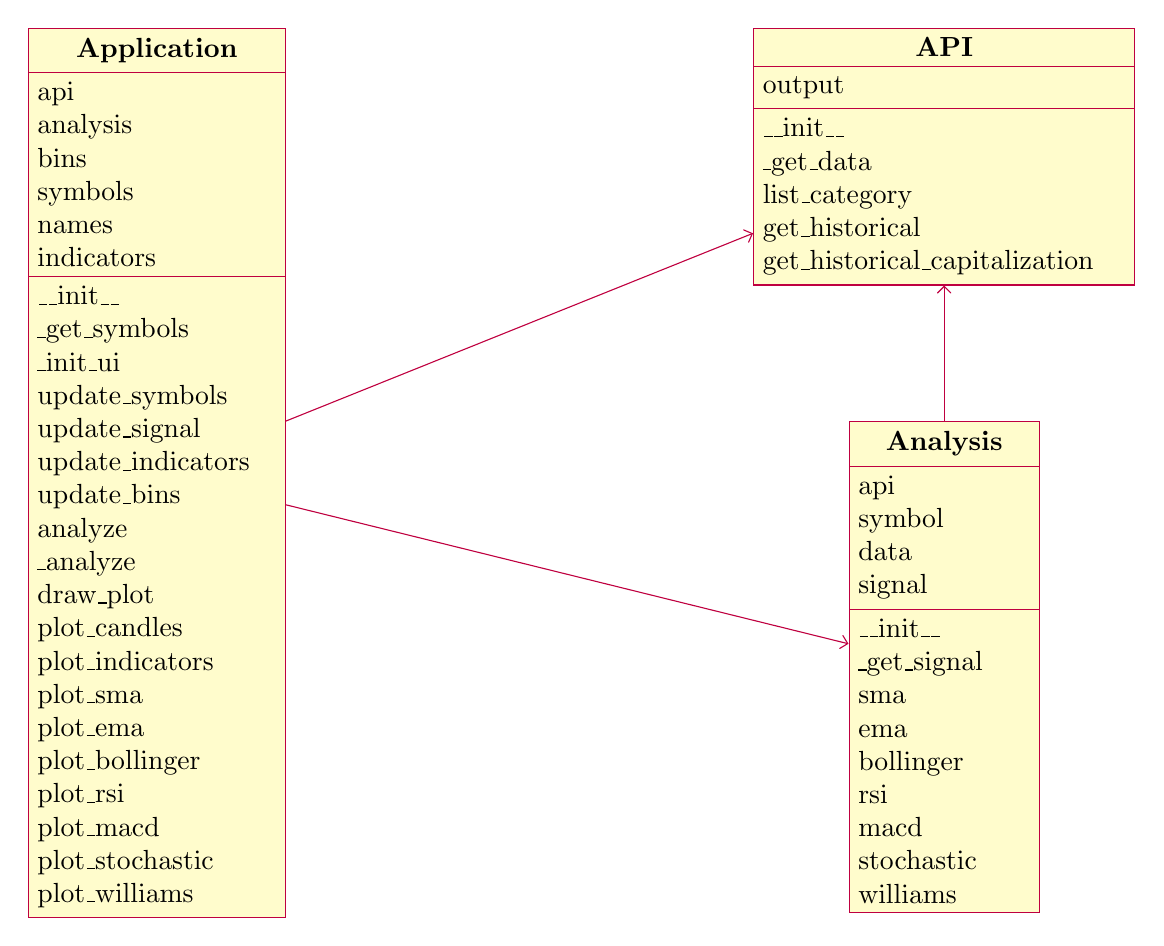
\begin{tikzpicture}
		\begin{class}[text width = 0.38\textwidth]{API}{10, 0}
			\attribute{output}
			\operation{\_\_init\_\_}
			\operation{\_get\_data}
			\operation{list\_category}
			\operation{get\_historical}
			\operation{get\_historical\_capitalization}
		\end{class}
		\begin{class}[text width = 0.18\textwidth]{Analysis}{10, -5}
			\attribute{api}
			\attribute{symbol}
			\attribute{data}
			\attribute{signal}
			\operation{\_\_init\_\_}
			\operation{\_get\_signal}
			\operation{sma}
			\operation{ema}
			\operation{bollinger}
			\operation{rsi}
			\operation{macd}
			\operation{stochastic}
			\operation{williams}
		\end{class}
		\begin{class}[text width = 0.25\textwidth]{Application}{0, 0}
			\attribute{api}
			\attribute{analysis}
			\attribute{bins}
			\attribute{symbols}
			\attribute{names}
			\attribute{indicators}
			\operation{\_\_init\_\_}
			\operation{\_get\_symbols}
			\operation{\_init\_ui}
			\operation{update\_symbols}
			\operation{update\_signal}
			\operation{update\_indicators}
			\operation{update\_bins}
			\operation{analyze}
			\operation{\_analyze}
			\operation{draw\_plot}
			\operation{plot\_candles}
			\operation{plot\_indicators}
			\operation{plot\_sma}
			\operation{plot\_ema}
			\operation{plot\_bollinger}
			\operation{plot\_rsi}
			\operation{plot\_macd}
			\operation{plot\_stochastic}
			\operation{plot\_williams}
		\end{class}
		
		\unidirectionalAssociation{Application}{}{}{Analysis}
		\unidirectionalAssociation{Application}{}{}{API}
		\unidirectionalAssociation{Analysis}{}{}{API}
		
	\end{tikzpicture}

\newpage
	\section{Opis interfejsu}\label{sec:opis-interfejsu}

	Aplikacja po uruchomieniu wygląda następująco:

	\begin{figure}[H]
		\centering
		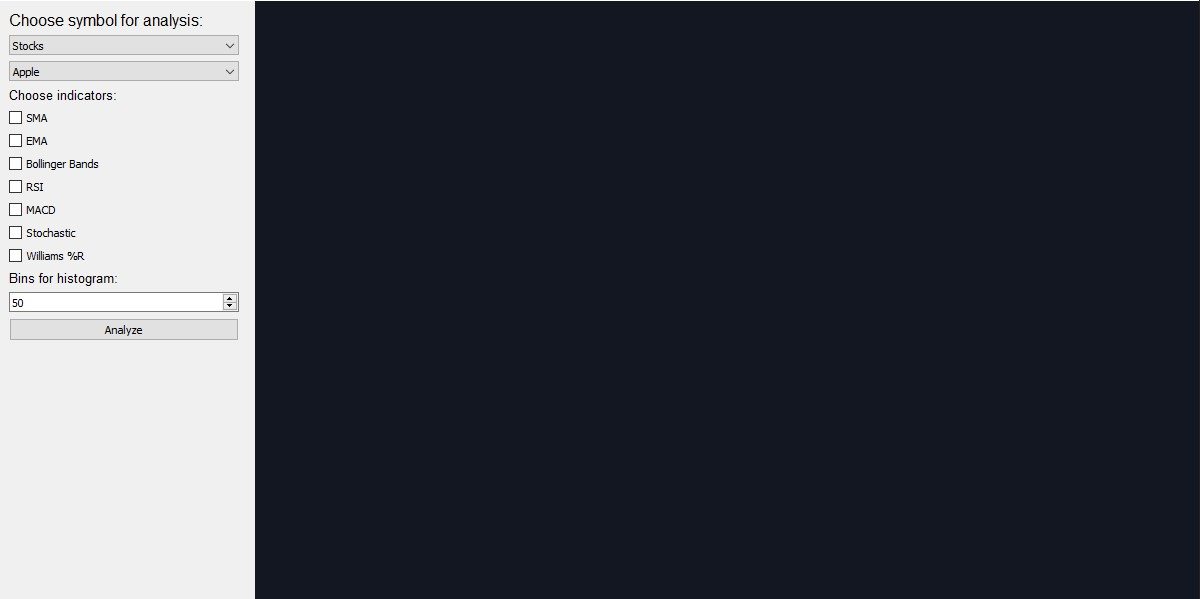
\includegraphics[scale=0.4]{pics/po_odpaleniu.jpg}
		\caption{Okno aplikacji po uruchomieniu} 
	\end{figure}
	
	Użytkownik ma możliwość modyfikowania opcji oznaczonych na poniższym rysunku numerami od 1 do 4.
	
	\begin{figure}[H]
		\centering
		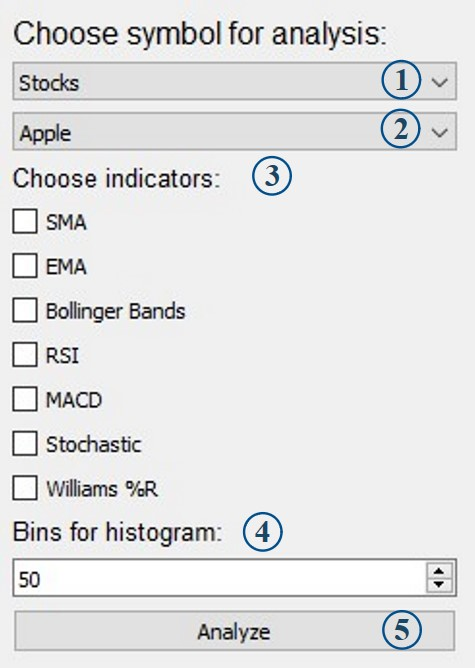
\includegraphics[scale=0.4]{pics/opcje.jpg}
		\caption{Dostępne opcje} 
	\end{figure}
	
	Użytkownik wybiera, jakim notowaniom chce się przyjrzeć. Dostępne opcje to: rynek akcyjny, rynek walutowy, rynek kryptowalut oraz rynek surowców. Może to zrobić modyfikując parametry oznaczone na powyższym rysunku numerami 1 i 2. Wybierając rynek akcyjny (1) można wybierać spośród akcji stu najpopularniejszych firm (2). 
	
	\begin{figure}[H]
		\centering
		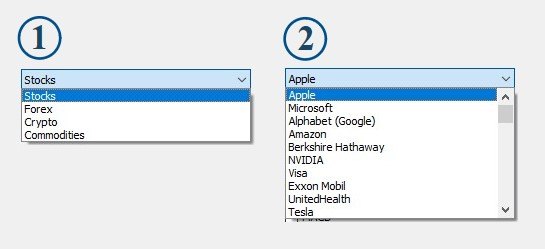
\includegraphics[scale=0.7]{pics/opcje_12.jpg}
		\caption{Dostępne parametry} 
	\end{figure}
	
	\begin{figure}[H]
		\centering
		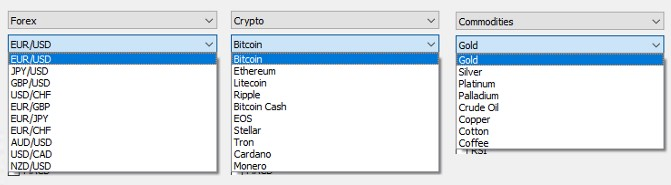
\includegraphics[scale=0.7]{pics/forex_crypto_commodities.jpg}
		\caption{Dostępne parametry dla pozostałych rynków}
	\end{figure}
	
	Następnie można wybrać wskaźniki (3), które zostaną uwzględnione na wykresie. Ich dokładny opis można znaleźć w sekcji \ref{wskazniki} tego dokumentu. Dostępne opcje to:
	
	\begin{itemize}
		\item SMA (ang. Simple Moving Average) - prosta średnia krocząca,
		\item EMA (ang. Exponential Moving Average) - wykładnicza średnia krocząca,
		\item Bollinger Bands - wstęgi Bollingera,  
		\item RSI (ang. Relative Strength Index) - wskaźnik siły względnej,
		\item MACD (ang. Moving Average Convergence Divergence) - konwergencja/dywergencja średnich kroczących,
		\item Stochastic - oscylator stochastyczny,
		\item Williams \%R - \%R Williamsa.
	\end{itemize}
	
	Ostatnim parametrem jest liczba świec na wykresie oznaczająca także liczbę dni, sprzed których dane nas interesują. Służy do tego opcja "Bins for histogram" (oznaczona numerem 4 na rysunku 2), która domyślnie przyjmuje wartość 50.\\
	
	\textbf{Uwaga:} ze względu na różniące się skale, niektóre kombinacje wskaźników są zablokowane!
	
	\begin{itemize}
		\item Wskaźnik RSI blokuje możliwość wyboru MACD.
		\item MACD blokuje wskaźniki RSI, Stochastic i Williams \%R.
		\item Stochastic i Williams \%R blokują wskaźnik MACD.	
	\end{itemize}
	
	Po kliknięciu przycisku "Analyze", oznaczonego numerem 5 na rysunku 2, otrzymujemy interesujący nas wykres. W lewym dolnym rogu okna wyświetla się również jedną z poniższych predykcji dotyczących inwestycji. 
	
	\begin{figure}[H]
		\centering
		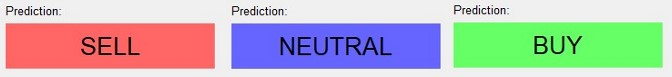
\includegraphics[scale=0.5]{pics/predykcje.jpg}
		\caption{Możliwe predykcje} 
	\end{figure}
	
	Predykcja SELL oznacza, że zalecana jest sprzedaż posiadanych akcji. W przypadku NEUTRAL, nie obserwuje się ani tendencji wzrostowej, ani spadkowej cen akcji. Decyzja o kupnie/sprzedaży akcji byłaby niewiadomą. BUY natomiast sugeruje, że inwestycja będzie dobrym posunięciem.\\

\newpage
	Przykładowo wygenerowana analiza prezentuje się następująco:
	
	\begin{figure}[H]
		\centering
		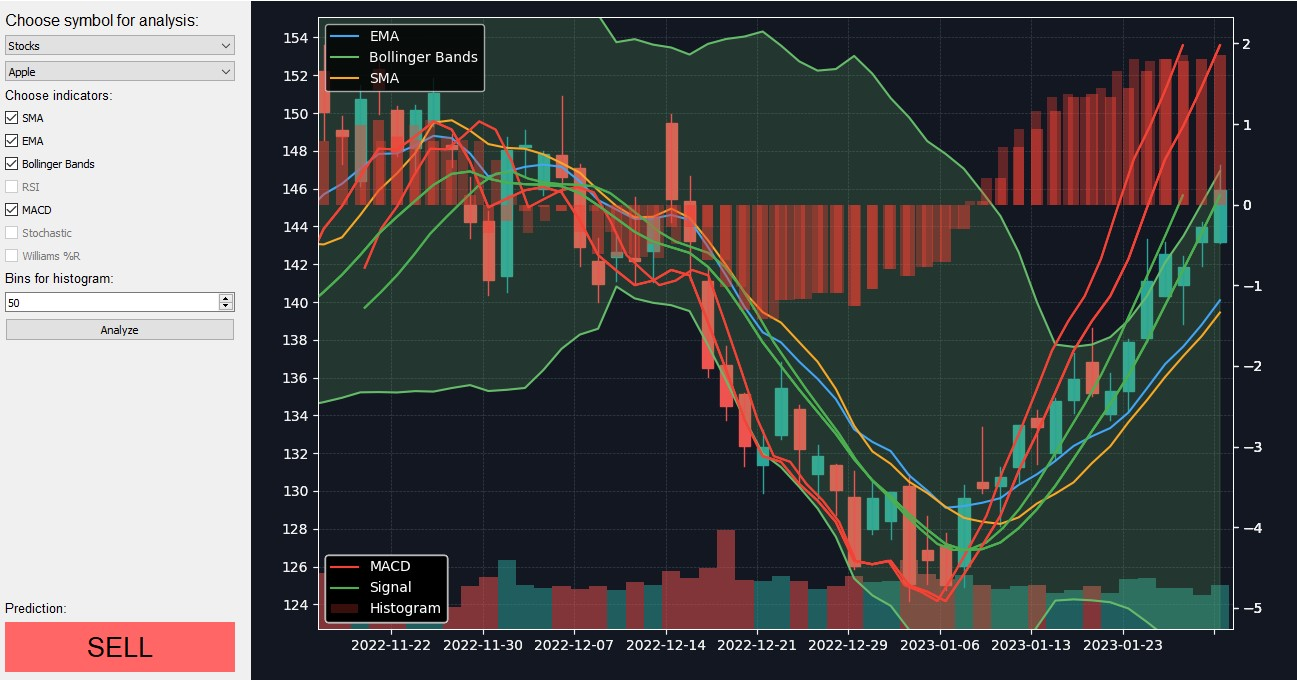
\includegraphics[scale=0.4]{pics/wykres.jpg}
		\caption{Przykładowy wykres z predykcją} 
	\end{figure}

\end{document}
